\documentclass[../../main.tex]{subfiles}

\begin{document}

\subsection{Mapping on Requirements}
\begin{itemize}
		\item \textbf{G1}:Allow policy maker to get information provided by the farmers about their production.
		
    		---\textbf{ R1}:The system shall allow an unregistered policy maker to register.
    		
    		---\textbf{ R2}:The system should be able to store the production information offered by farmers.
    		
    		---\textbf{ R3}:The system should allow policy makers to extract the production information.
    		
    		---\textbf{ R4}:The system should get farmers' GPS information and weather conditions there to show to policy makers.
    		
		    ---\textbf{ D3}:All farmers are truthful and regularly upload their production.
		    
    		---\textbf{ D3}:All farmers are truthful and regularly upload their production.
    		
    		---\textbf{ D7}:All DREAM users have an IT device with support for Internet connectivity or a standard telephone line.
		
		
		\item \textbf{G2}:Allow policy maker to get farmers’ production ranking.
		    
		    ---\textbf{ R3}:The system should allow policy makers to extract the production information.
		    
		    ---\textbf{ R4}:The system should get farmers' GPS information and weather conditions there to show to policy makers.
		    
		    ---\textbf{ R5}:The system should ranking farmers' production and show to policy makers.
		    
		    ---\textbf{ R6}:The system should let policy makers know how to contact each farmer.
		    
    		---\textbf{ D7}:All DREAM users have an IT device with support for Internet connectivity or a standard telephone line.
		
		
		\item \textbf{G3}:Allow farmers to get relevant weather forecasts and suggestions based on the farmer’s location and production information.
		
		    ---\textbf{ R7}:The system shall allow an unregistered farmer to register.
		    
		    ---\textbf{ R8}:After the farmer has successfully entered all the information required for registration, the system will send him/her a cell phone verification code to complete the registration process.
		    
		    ---\textbf{ R9}:The system must remember each farmers' field location.
		    
    		---\textbf{ D1}:The number of policy makers is sufficient to identify and reward all farmers who rank high.
    		
    		---\textbf{ D2}:Policy makers will help every farmer who asks for help.
    		
    		---\textbf{ D4}:All farmers will allow the software to access farm location information.
		
		
		\item \textbf{G4}:Allow farmers to upload their production and problems.
		
		    ---\textbf{ R10}:The system must remember each farmers' problems data.
		    
		    ---\textbf{ R11}:The system must allow farmers to upload different type of problem, such as picture, text and video.
		    
		    ---\textbf{ R12}:The system shall rank problems by uploading time.
		    
		    ---\textbf{ R13}:The system shall allow farmers to delete their problems on forums.
		    
		    ---\textbf{ D7}:All DREAM users have an IT device with support for Internet connectivity or a standard telephone line.
		
		
		\item \textbf{G5}:Allow farmers to create discussion forums with the other farmers.
		
            ---\textbf{ R14}:The system will allow all farmers and all agronomist having access to all problems.
		    
		    ---\textbf{ D7}:All DREAM users have an IT device with support for Internet connectivity or a standard telephone line.
		
		
		\item \textbf{G6}:Allow farmers to respond to other farmers’ questions.
		
		    ---\textbf{ R13}:The system shall allow farmers to delete their problems on forums.
		    
		    ---\textbf{ R14}:The system will allow all farmers having access to all problems.
		    
		    ---\textbf{ D5}:Farmers will answer questions they know in the forum.
		    
		    ---\textbf{ D7}:All DREAM users have an IT device with support for Internet connectivity or a standard telephone line.
		
		
		\item \textbf{G7}:Allow agronomists to respond to the farmers’ questions.
		    
		    ---\textbf{ R15}:The system will allow an unregistered Agronomist to register..
		    
		    ---\textbf{ R16}:After the agronomist has successfully entered all the information required for registration, the system will send him/her a cell phone verification code to complete the registration process.
		    
		    ---\textbf{ R17}:The system will allow all agronomists to respond to the farmers’ questions.
		    
		     ---\textbf{ R18}:The system will allow all agronomists to have access to all farmer's detail information such as production, location weather and so on.
		     
		      ---\textbf{ R17}:The system will allow all agronomists to respond to the farmers’ questions.
		    
		    ---\textbf{ D3}:All farmers are truthful and regularly upload their production.
		    
		    ---\textbf{ D6}:Agronomists will provide adequate help to farmers who need it.
		    
		    ---\textbf{ D7}:All DREAM users have an IT device with support for Internet connectivity or a standard telephone line.

\end{itemize}

\subsection{Use case diagrams}
\begin{itemize}
    

    \item \textbf{unregistered policy maker}
    
      \begin{figure}[H]
        \centering
        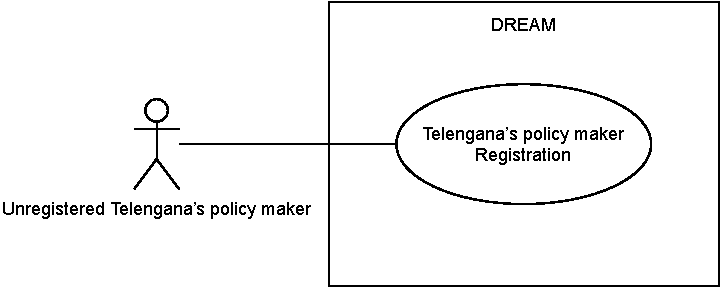
\includegraphics[width=\textwidth]{RASD/image/Use_Cases2_policy_maker.pdf}
      \end{figure}
      
      
      
    \item \textbf{unregistered farmer}
    
      \begin{figure}[H]
        \centering
        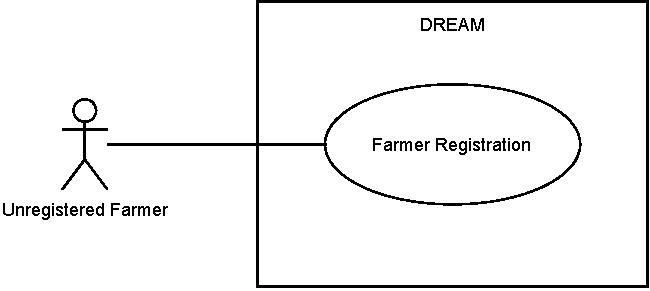
\includegraphics[width=\textwidth]{RASD/image/Use_Cases_farmer.pdf}
      \end{figure}
      
      
      
    \item \textbf{unregistered agronomist}
    
      \begin{figure}[H]
        \centering
        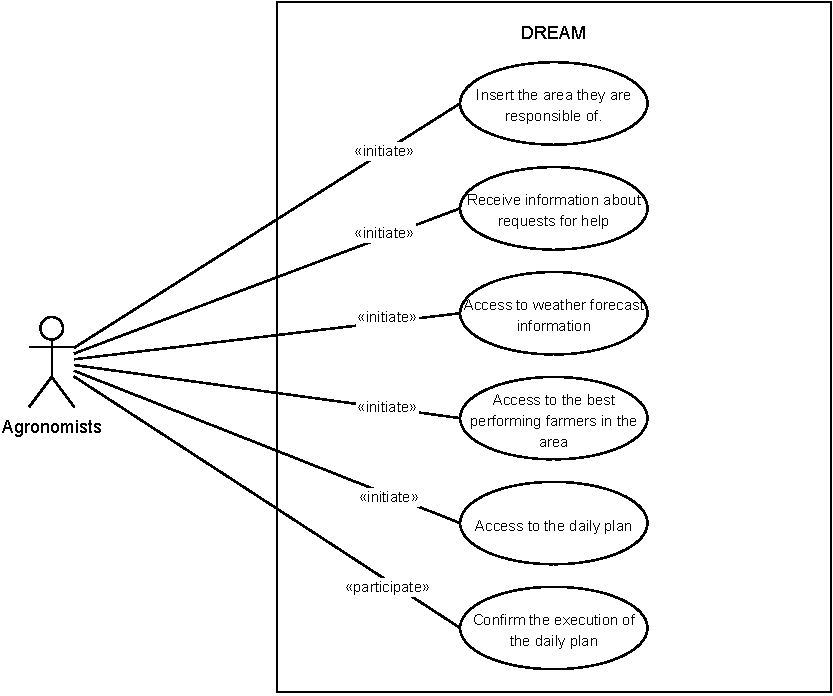
\includegraphics[width=\textwidth]{RASD/image/Use_Cases_Application_Agronomists.drawio.pdf}
      \end{figure}
      
      
      
    \item \textbf{application policy maker}
    
      \begin{figure}[H]
        \centering
        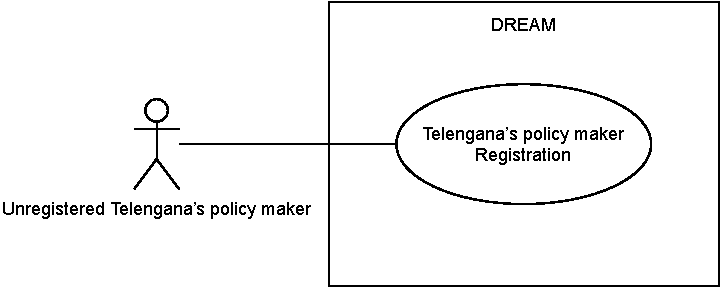
\includegraphics[width=\textwidth]{RASD/image/Use_Cases2_policy_maker.pdf}
      \end{figure}
      
      
      
    \item \textbf{application farmer}
    
      \begin{figure}[H]
        \centering
        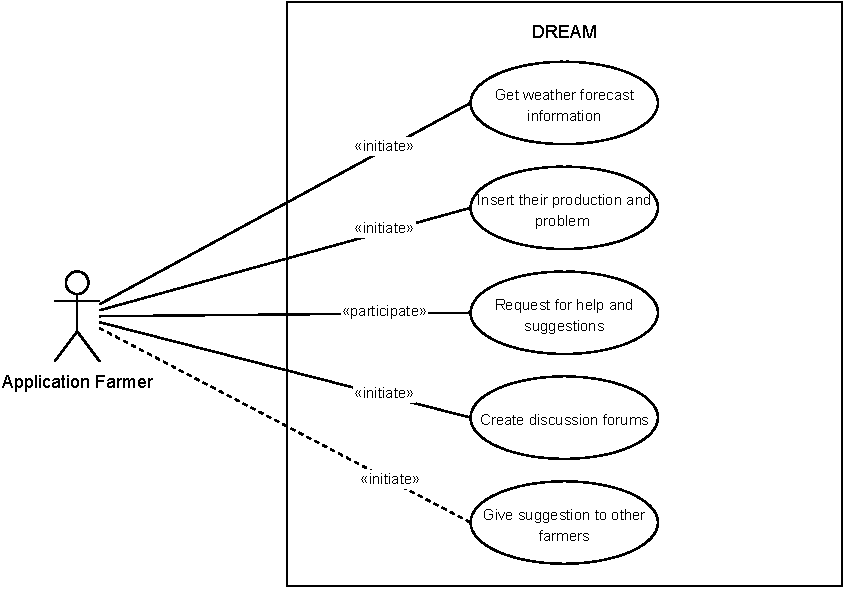
\includegraphics[width=\textwidth]{RASD/image/Use_Cases_Application_farmer.drawio.pdf}
      \end{figure}
      
      
      
    \item \textbf{application agronomist}

      \begin{figure}[H]
        \centering
        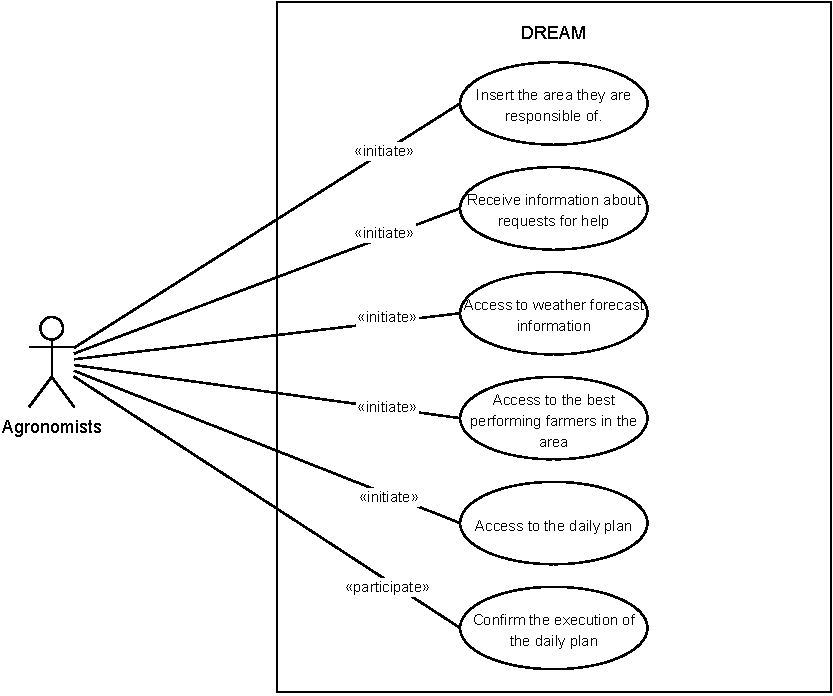
\includegraphics[width=\textwidth]{RASD/image/Use_Cases_Application_Agronomists.drawio.pdf}
      \end{figure}



\end{itemize}


\subsection{Use cases and Sequence diagrams}
      \subsubsection{Policy maker registration}
      \begin{table}[H]
        \centering
          \begin{tabular}{c m{.75\textwidth}}
          \hline
          \textbf{Use Case} & Policy maker registration\\ \hline
          \textbf{Actor} & Policy maker\\ \hline
          \textbf{Entry condition} & Policy maker wants to use DREAM system to manage farmers.\\  \hline
          \textbf{Flow of events} & \begin{itemize}
                                      \item Policy maker start to sign up.
                                      \item The system shows sign up view.
                                      \item Policy maker create credentials(username, password)
                                      \item The system will check username if it is available.
                                      \item The system shows to policy makers user details
                                      \item Policy maker confirm sign up.
                
                                    \end{itemize}\\ \hline
          \textbf{Exit condition} & The system shows a confirmation message to policy maker. \\ \hline
          \textbf{Exceptions} &  If the username has been used by other policy maker, system will let you to change another username.\\ 
          \hline
          \end{tabular}
      \end{table}

      \begin{figure}[H]
        \centering
        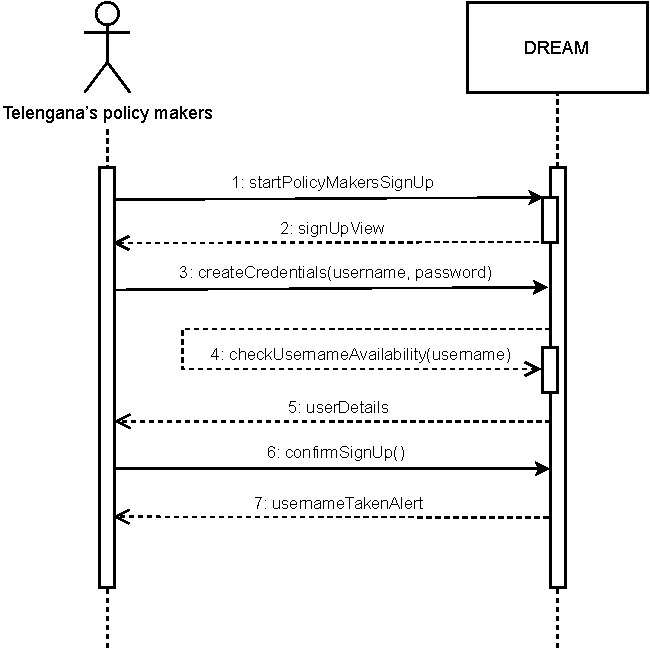
\includegraphics[width=\textwidth]{RASD/image/Sequence_Diagram_Policy_maker.pdf}
        \caption{Policy maker registration sequence diagram}
      \end{figure}

      \subsubsection{Farmer registration}

      \begin{table}[H]
        \centering
          \begin{tabular}{c m{.75\textwidth}}
          \hline
          \textbf{Use Case} & Farmer registration\\ \hline
          \textbf{Actor} & Farmer\\ \hline
          \textbf{Entry condition} & The farmer wants to use DREAM.\\  \hline
          \textbf{Flow of events} & \begin{itemize}
                                     \item The farmer start to sign up.
                                      \item The system shows sign up view.
                                      \item The farmer create credentials(username, password)
                                      \item The system will check username if it is available.
                                      \item The system shows to farmer user details
                                      \item The farmer confirm sign up.
                                    \end{itemize}\\ \hline
          \textbf{Exit condition} & The system shows a confirmation message to farmer \\ \hline
          \textbf{Exceptions} & If the username has been used by other farmer, system will let you to change another username. \\ \hline
          \end{tabular}
      \end{table}

      \begin{figure}[H]
        \centering
        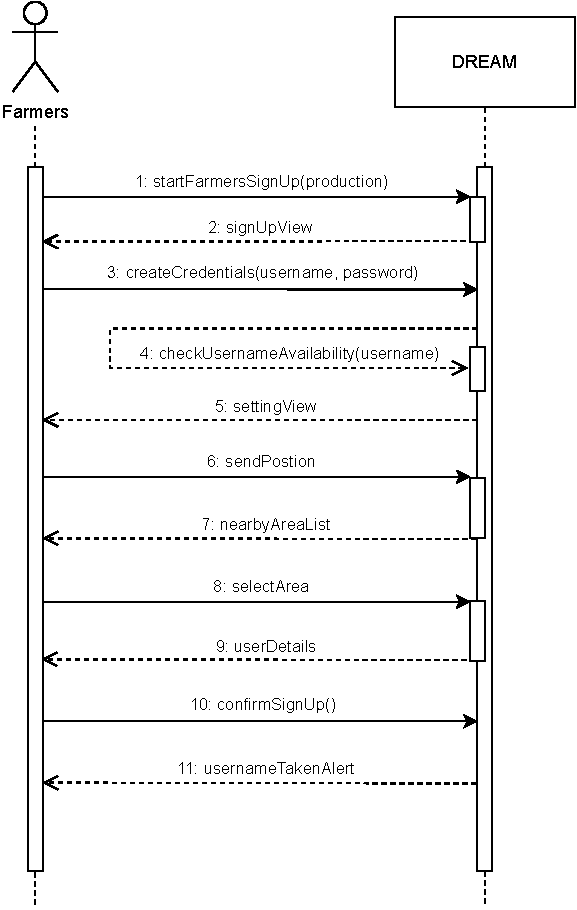
\includegraphics[width=13cm]{RASD/image/Sequence_Diagram_Farmers.pdf}
        \caption{Farmer registration sequence diagram}
      \end{figure}


      \subsubsection{Agronomist registration}

      \begin{table}[H]
        \centering
          \begin{tabular}{c m{.75\textwidth}}
          \hline
          \textbf{Use Case} & Agronomist registration\\ \hline
          \textbf{Actor} & Agronomist\\ \hline
          \textbf{Entry condition} & A customer wants to cancel their reservation\\  \hline
          \textbf{Flow of events} & \begin{itemize}
                                     \item The agronomist start to sign up.
                                      \item The system shows sign up view.
                                      \item The agronomist create credentials(username, password)
                                      \item The system will check username if it is available.
                                      \item The agronomist will send his/her location to DREAM.
                                      \item The system will send a nearby List to agronomist.
                                      \item The agronomist will choose a certain Area.
                                      \item The system shows to agronomist user details
                                      \item The agronomist confirm sign up.
                                    \end{itemize}\\ \hline
          \textbf{Exit condition} & The system shows a confirmation message to agronomist \\ \hline
          \textbf{Exceptions} & If the username has been used by other agronomist, system will let you to change another username.\\ \hline
          \end{tabular}
      \end{table}

      \begin{figure}[H]
        \centering
        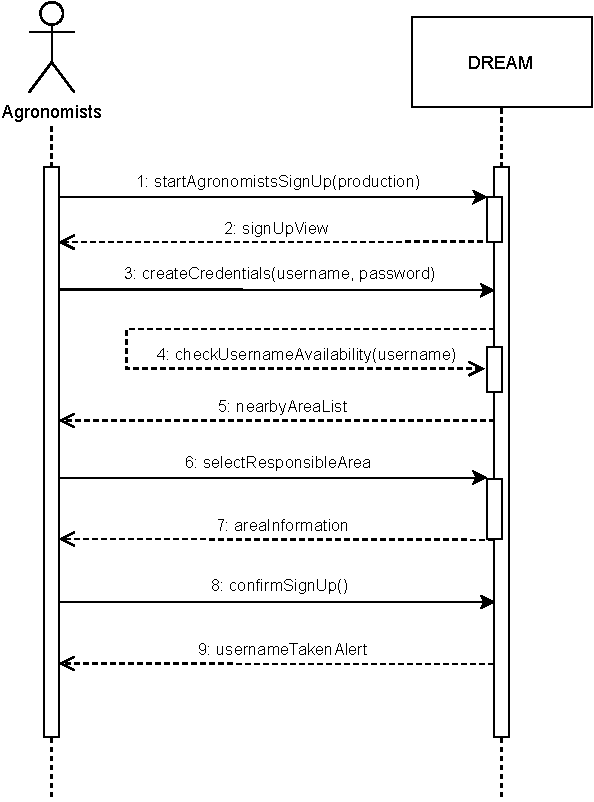
\includegraphics[width=\textwidth]{RASD/image/Sequence_Diagram_Agronomists.pdf}
        \caption{Agronomist registration sequence diagram}
      \end{figure}

      
      \subsubsection{Identify Good Farmers}

      \begin{table}[H]
        \centering
          \begin{tabular}{c m{.75\textwidth}}
          \hline
          \textbf{Use Case} & Identify Good Farmers\\ \hline
          \textbf{Actor} & Policy makers\\ \hline
          \textbf{Entry condition} & Policy maker wants to know which farmer done will at their production\\  \hline
          \textbf{Flow of events} & \begin{itemize}
                                      \item Policy maker open ranking page.
                                      \item The system shows to policy maker which farmer performing well, and shows their information.
                                    \end{itemize}\\ \hline
          \textbf{Exit condition} & Policy maker got information about well-performing farmers. \\ \hline
          \textbf{Exceptions} & \\ \hline
          \end{tabular}
      \end{table}

      \begin{figure}[H]
        \centering
        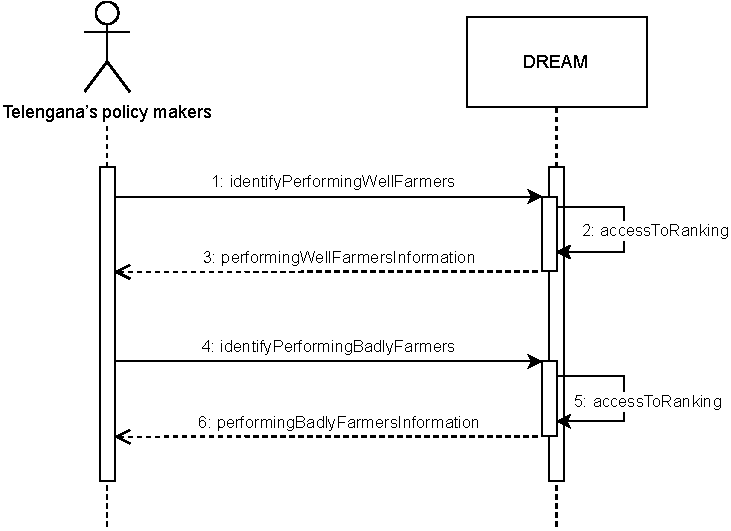
\includegraphics[width=\textwidth]{RASD/image/Sequence_Diagram_Policy_maker-IdetifyGoodFarmers.drawio.pdf}
        \caption{Identify Good Farmers sequence diagram}
      \end{figure}


      \subsubsection{Judgement result}

      \begin{table}[H]
        \centering
          \begin{tabular}{c m{.75\textwidth}}
          \hline
          \textbf{Use Case} & Judgement result \\ \hline
          \textbf{Actor} & Policy makers\\ \hline
          \textbf{Entry condition} & Policy maker wants to know the  production of farmers who was helped by other farmers or agronomist.\\  \hline
          \textbf{Flow of events} & \begin{itemize}
                                      \item Policy maker wants to know the production of farmers who was helped by other farmers or agronomist.
                                    \end{itemize}\\ \hline
          \textbf{Exit condition} & The policy maker got information. \\ \hline
          \textbf{Exceptions} & \\ \hline
          \end{tabular}
      \end{table}

      \begin{figure}[H]
        \centering
        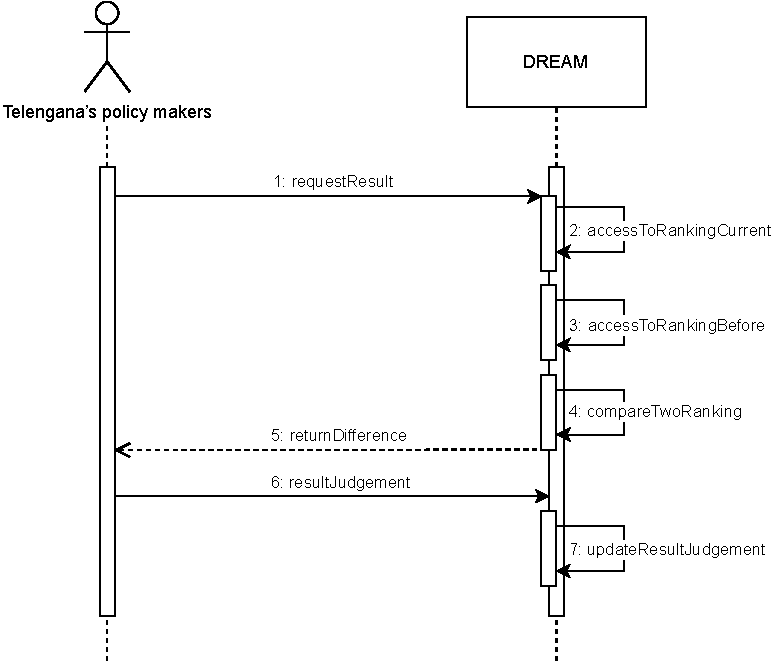
\includegraphics[width=\textwidth]{RASD/image/Sequence_Diagram_Policy_maker-ResultJudgement.drawio.pdf}
        \caption{Judgement result sequence diagram}
      \end{figure}


      \subsubsection{Request for suggestions}

      \begin{table}[H]
        \centering
          \begin{tabular}{c m{.75\textwidth}}
          \hline
          \textbf{Use Case} & Request for suggestions \\ \hline
          \textbf{Actor} & Farmers\\ \hline
          \textbf{Entry condition} & The farmer needs to be helped at DREAM.\\  \hline
          \textbf{Flow of events} & \begin{itemize}
                                      \item The farmer needs to be helped on DREAM and he/she write problems information on DREAM.
                                      \item The system shows available suggestion way.
                                      \item Farmer request suggestions.
                                      \item The system returns suggestions.
                                    \end{itemize}\\ \hline
          \textbf{Exit condition} & Farmer complete request-suggestions processing. \\ \hline
          \textbf{Exceptions} &  \\ \hline
          \end{tabular}
      \end{table}

      \begin{figure}[H]
        \centering
        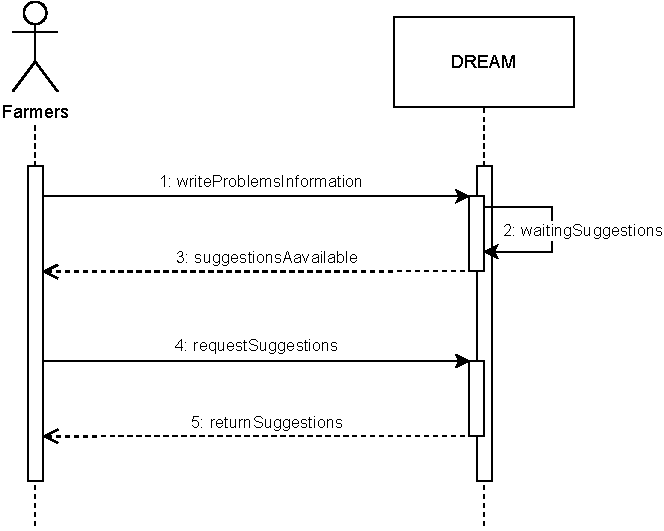
\includegraphics[width=\textwidth]{RASD/image/Sequence_Diagram_Farmers-requestForSuggestions.drawio.pdf}
        \caption{Request for suggestions sequence diagram}
      \end{figure}


      \subsubsection{Create discussion}

      \begin{table}[H]
        \centering
          \begin{tabular}{c m{.75\textwidth}}
          \hline
          \textbf{Use Case} & Create discussion\\ \hline
          \textbf{Actor} & Farmers\\ \hline
          \textbf{Entry condition} & Farmer wants to discuss something with other farmers shopping. \\  \hline
          \textbf{Flow of events} & \begin{itemize}
                                      \item Farmer starts create discussion forums
                                      \item  select Participants And Topic
                                    \end{itemize}\\ \hline
          \textbf{Exit condition} & Farmers finished create discuss. \\ \hline
          \textbf{Exceptions} & \\ \hline
          \end{tabular}
      \end{table}

      \begin{figure}[H]
        \centering
        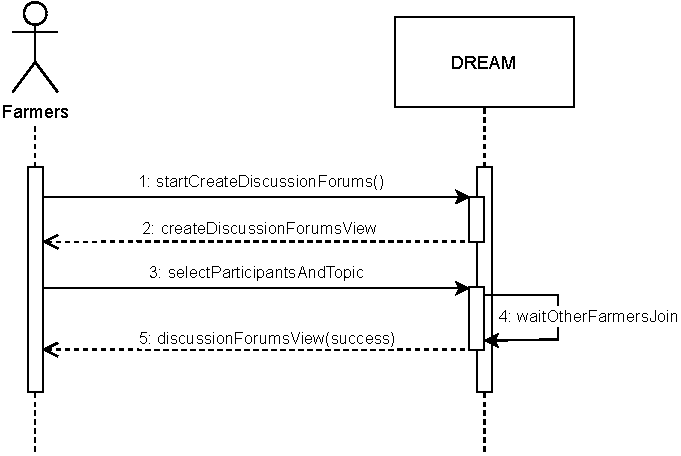
\includegraphics[width=\textwidth]{RASD/image/Sequence_Diagram_Farmers-create discussion.pdf}
        \caption{Create discussion sequence diagram}
      \end{figure}


      \subsubsection{Access to data}

      \begin{table}[H]
        \centering
          \begin{tabular}{c m{.75\textwidth}}
          \hline
          \textbf{Use Case} & Access to data\\ \hline
          \textbf{Actor} & Farmers\\ \hline
          \textbf{Entry condition} & A customer asks a store assistant for a line up receipt\\  \hline
          \textbf{Flow of events} & \begin{itemize}
                                      \item Farmers have access to weather data.
                                      \item Farmers need to acquire weather data.
                                      \item The system return weather data.
                                      \item Farmers have access to suggestions(location, production Type)
                                      \item Farmers acquire Personalized Suggestions
                                      \item The system return suggestions.
                                    \end{itemize}\\ \hline
          \textbf{Exit condition} & Farmers got suggestions.\\ \hline
          \textbf{Exceptions} & \\ \hline
          \end{tabular}
      \end{table}

      \begin{figure}[H]
        \centering
        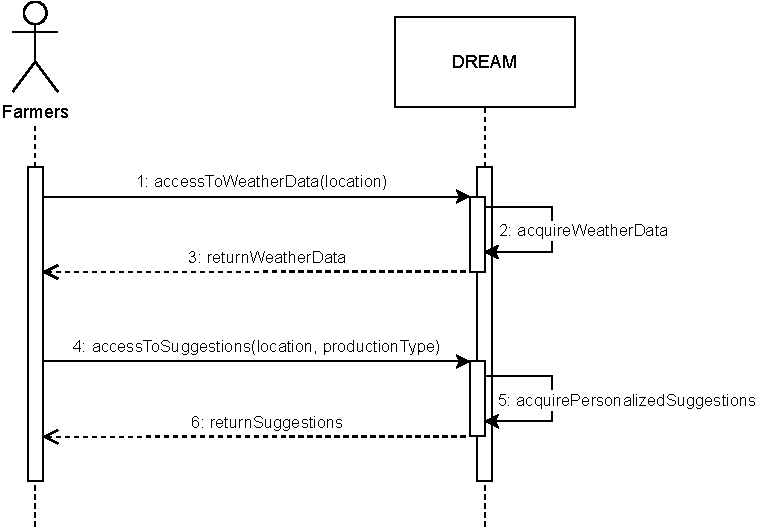
\includegraphics[width=\textwidth]{RASD/image/Sequence_Diagram_Farmers-accessToData.pdf}
        \caption{Access to data sequence diagram}
      \end{figure}


      \subsubsection{Daily plan}

      \begin{table}[H]
        \centering
          \begin{tabular}{c m{.75\textwidth}}
          \hline
          \textbf{Use Case} & Daily plane\\ \hline
          \textbf{Actor} & Agronomists\\ \hline
          \textbf{Entry condition} & Agronomist needs to manage his/her system.\\  \hline
          \textbf{Flow of events} & \begin{itemize}
                                      \item Agronomists request Daily Plan.
                                      \item The system will return visit list.
                                      \item Agronomists have access To Ranking.
                                      \item Agronomists can confirm The Execution.
                                      \item The system shows daily plan view.
                                      \item Agronomists can specify his/her deviations.
                                      
                                    \end{itemize}\\ \hline
          \textbf{Exit condition} & Agronomist finish his/her tasks \\ \hline
          \textbf{Exceptions} & \\ \hline
                              \end{tabular}
      \end{table}

      \begin{figure}[H]
        \centering
        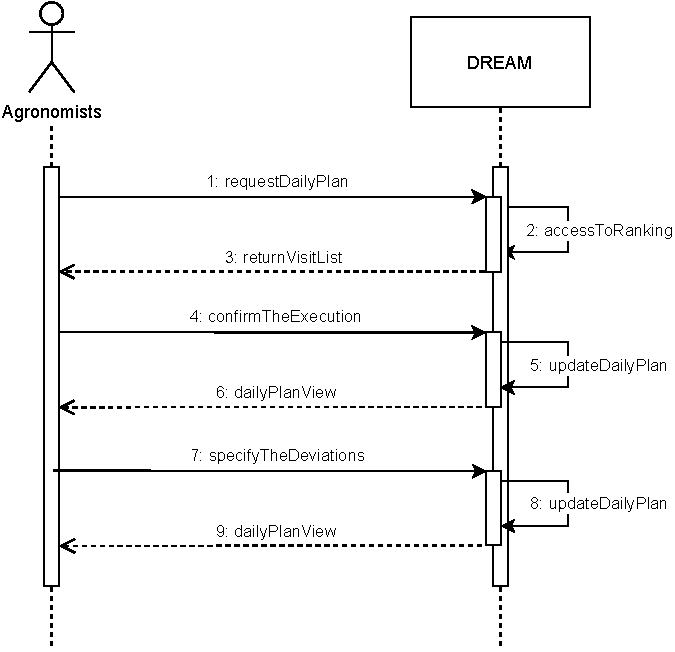
\includegraphics[width=\textwidth]{RASD/image/Sequence_Diagram_Agronomists-DailyPlan.drawio.pdf}
        \caption{Daily plan sequence diagram}
      \end{figure}

\end{document}
